\documentclass{article}
\usepackage[utf8]{inputenc}
\usepackage[T1]{fontenc}
\usepackage{amsmath}
\usepackage{amsfonts}
\usepackage{amssymb}
\usepackage{amssymb, bm}
\usepackage{mathtools, bm}
\usepackage{mathrsfs}
\usepackage{stmaryrd}
\usepackage{graphicx}
\usepackage{tikz}
%\usepackage[]{algorithm2e}
\usepackage[]{algorithm}
\usepackage[]{algorithmic}

% fonction pour définir une fonction 
\newcommand{\fonction}[5]{
	\begin{array}{ccccc}
#1 & : & #2 & \to & #3\\
	& & #4 & \mapsto & #5\\ 
	\end{array}
}

\begin{document}
\section{Introduction}
L'apprentissage profond est une branche du machine learning. Dans cette branche, nous trouvons des algorithmes qu'on utilise principalement dans la reconnaissance d'image et vocal et qui est capable d'apprendre de manière autonome ou supervisé. Notre projet consiste à utiliser l'apprentissage profond dans le problème des formules quantifiées booléenne (dit QBF). Les formules booléennes quantifiées permettent de modéliser de nombreuses situations de la vie courante. Une des questions que nous pouvons nous poser est de savoir si celles-ci sont satisfaisable ou non. Cette question est un grand problème dans l'informatique théorique qu'on place dans la classe PSPACE-complet. Le fait d'utiliser l'apprentissage profond afin de savoir si une formule QBF est satisfaisable est très peu commun et reste une démarche expérimental. Dans ce rapport, nous allons premièrement parler des outils de base qu'on utilise dans l'apprentissage profond qui sont les neurones et réseaux de neurones. Nous allons ensuite voir la notions clef de ce domaine qui est l'apprentissage. Nous terminerons ce rapport en parlant de notre démarche expérimental qui
sera un algorithme permettant de vérifier la satisfaisabilitée d'une formule QBF.  
\newpage

\section[Titre plus court]{Les Neurones}
Le premier modèle mathématique et informatique du neurone biologique a été donné par Warren McCulloh et Walter Pitts en 1943.
Ce modèle inspiré de la neurobiologie, fait intervenir n entrées auxquelles des fonctions y seront appliquées afin d'en obtenir une sortie.
Voici une définition plus formelle de ce modèle qu'on nomme: Modèle de McCulloh-Pitts     

\subsection{Définition: Modèle de McCulloh-Pitts}
	Soit la fonction  

	\[\fonction{\varphi}{\mathbb{R}^n}{\left\{0,1\right\}}{(x_1,....,x_n)}{\varphi(x_1,....,x_n)} \]

	tel que  
	\[\varphi (x_1,...,x_n) = g(f(x_1,....,x_n)). \]  

	\begin{enumerate}
		\item $f$ est définie comme étant la fonction somme 
		\[\fonction{f}{\mathbb{R}^n}{\mathbb{R}}{(x_1,....,x_n)}{\sum_{i=1}^{n} {x_i}} \] 
		\item On appelle $g$ la fonction d'activation à seuil. Celle-ci est définie de la manière suivante :

		\[g(x) = \begin{cases} 0 &\mbox{Si } x < \theta \\
				 1 & \mbox{Si } x \geq \theta
	 		 \end{cases} 
		\]
	\end{enumerate}

%**************************************************************************************% 
% code pour la figure 2

\vfill
\begin{center}
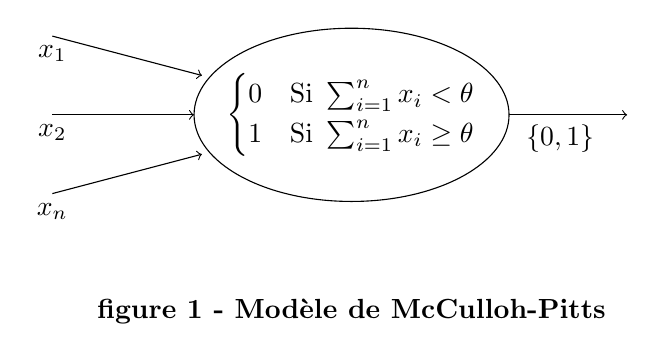
\begin{tikzpicture}[]
	%\draw[help lines, thick] (0,0) grid (9,5);
	\draw[->] (0.7,2.5) node [below] {$x_{2}$}-- (2.5,2.5);
	\draw[->] (6.5,2.5)-- node[below, align=center] {$\left\{0,1\right\}$} (7.8,2.5)-- (8,2.5);
	\draw[->] (0.7,3.5) node [below] {$x_{1}$} -- (2.6,3);
	\draw[->] (0.7,1.5) node [below] {$x_{n}$}-- (2.6,2);
	\draw (4.5,2.5) node {$ \begin{cases} 0 &\mbox{Si } \sum_{i=1}^{n} {x_i} < \theta \\ 1 & \mbox{Si } \sum_{i=1}^{n} {x_i} \geq \theta \end{cases} $} circle [x radius= 2, y radius=1.1];
	\draw (4.5,0) node { \textbf{figure 1 - Modèle de McCulloh-Pitts} };
\end{tikzpicture}
\end{center}
\vfill
%**************************************************************************************% 

\textbf{Remarque} : La valeur $\theta$  qu'on utilise dans la fonction $g$ est appelée le seuil.\\
	

Le modèle de McCulloh-Pitts a été décliné en de multiple manières au cours du temps. Les déclinaisons auxquelles nous allons nous intéresser sont appelées le modèle Perceptron et le modèle Sigmoid. Ces deux modèles introduisent la notion de poids qui est au cœur du processus d'apprentissage d'un réseau de neurone. 

\subsection{Définition: Modèle Perceptron}
		Le premier modèle du Perceptron a été introduit en 1958 par Frank Rosenblatt. Celui-ci a ensuite été repris et perfectionné dans les années soixante par Minsky et Papert. Ce modèle reprend la définition précédente sauf que pour chaque entrées $x_i$ ($i$ $\in$ $\llbracket 1~;~n \rrbracket$) on y associera une valeur (les fameux poids) $w_i$ $\in$ $\mathbb{R}$. 
		On définit alors la fonction $f$ de la façon suivante : 
		
		\[\fonction{f}{\mathbb{R}^n}{\mathbb{R}}{(x_1,....x_n)}{\sum_{i=1}^{n} {w_ix_i}}. \]

	
	\textbf{Remarque} : On note parfois \[b = -\theta \]  et on appel cette valeur le bias (ou inclinaison en français). La fonction $g$ est alors définit de la manière suivante :   
		\[g(x) = \begin{cases} 0 &\mbox{Si } x + b < 0 \\
				 1 & \mbox{Si } x + b \geq 0
	 		 \end{cases} \] \\
%**************************************************************************************% 
% code pour la figure 2
\vfill
\begin{center}
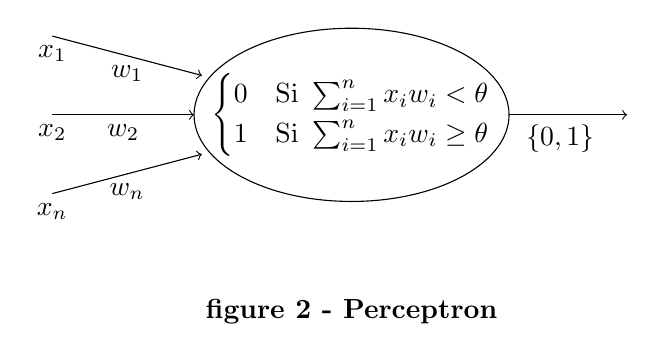
\begin{tikzpicture}[]
	%\draw[help lines, thick] (0,0) grid (9,5);
	\draw[->] (0.7,2.5) node [below] {$x_{2}$}-- node [below] {$w_{2}$} (2.5,2.5);
	\draw[->] (6.5,2.5)-- node[below, align=center] {$\left\{0,1\right\}$} (7.8,2.5)-- (8,2.5);
	\draw[->] (0.7,3.5) node [below] {$x_{1}$} -- node [below] {$w_{1}$} (2.6,3);
	\draw[->] (0.7,1.5) node [below] {$x_{n}$}-- node [below] {$w_{n}$} (2.6,2);
	\draw (4.5,2.5) node {$ \begin{cases} 0 &\mbox{Si } \sum_{i=1}^{n} {x_iw_i} < \theta \\ 1 & \mbox{Si } \sum_{i=1}^{n} {x_iw_i} \geq \theta \end{cases} $} circle [x radius= 2, y radius=1.1];
	\draw (4.5,0) node { \textbf{figure 2 - Perceptron} };
\end{tikzpicture}
\end{center}
\vfill
%**************************************************************************************% 
	 
Cette notion de poids va intervenir dans le processus d'apprentissage d'un réseau de neurone. Le but de ce processus, sera de trouver les bonnes valeurs à associer aux entrées afin que le réseau de neurone produise la meilleure sortie possible. Pour répondre au besoin du processus d'apprentissage, l'algorithme de la descente de gradient sera utilisé. Nous détaillerons plus tard cet algorithme mais le principe de celui-ci est d'ajuster petit à petit les poids afin d'affiner la sortie du réseau de neurone vers la valeur voulue. Cet affinement implique que la sortie $s$ $\in$ $\left[0,1\right]$, cependant la fonction $g$ ne sera  plus une fonction en escalier mais une fonction continue. Le Perceptron ne répondant plus à ces critères, le Sigmoid a été introduit. \\
% préciser le fait que avec une fonction en escalier il y a des gros saut et qu'avec une fonction continue il y a des petits sauts
% la particularitée ???
	\subsection{Définition: Modèle Sigmoid}
	 Le modèle Sigmoid est défini de la même manière que le modèle perceptron mais il y diffère à la fonction $g$. La fonction $g$ aura pour particularité d'être continue. On appelle cette fonction, la fonction sigmoid.  
		  \[ \fonction{g}{\mathbb{R}}{\left[0,1\right]}{x}{ \frac{1}{1+ e^{-x}}} \]


%**************************************************************************************% 
% code pour la figure 3 
\vfill
\begin{center}
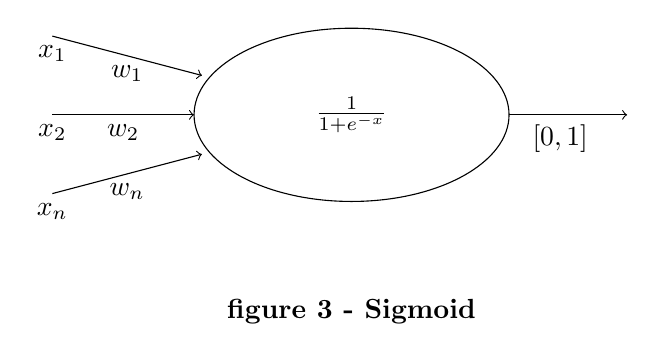
\begin{tikzpicture}[]
	%\draw[help lines, thick] (0,0) grid (9,5);
	\draw[->] (0.7,2.5) node [below] {$x_{2}$}-- node [below] {$w_{2}$} (2.5,2.5);
	\draw[->] (6.5,2.5)-- node[below, align=center] {$\left[0,1\right]$} (7.8,2.5)-- (8,2.5);
	\draw[->] (0.7,3.5) node [below] {$x_{1}$} -- node [below] {$w_{1}$} (2.6,3);
	\draw[->] (0.7,1.5) node [below] {$x_{n}$}-- node [below] {$w_{n}$} (2.6,2);
	\draw (4.5,2.5) node {$ \frac{1}{1+e^{-x}}  $} circle [x radius= 2, y radius=1.1];
	\draw (4.5,0) node { \textbf{figure 3 - Sigmoid} };
\end{tikzpicture}
\end{center}
\vfill
%**************************************************************************************% 
		
	\subsection{Définition: Réseau de Neurone}
 	Un réseau de neurone est un ensemble de neurones connectés entre eux. Ce réseau est composé de plusieurs couches : 
	\begin{enumerate}	
		\item la couche d'entrée : Cette couche est composée de neurones dont leurs entrées n'est pas la sortie d'autre neurone. 
		\item la couche cachée : Cette couche peut être composée de plusieurs couches de neurone. Les entrées des neurones sont les sorties de ceux de la couche précédente.
		\item la couche de sortie : Cette couche nous donne le résultat du réseau. Elle peut être formée d'un ou plusieurs neurone.
	\end{enumerate}		
% a faire un schéma pour le réseau de neurone 
		
	Nous avons défini dans cette partie qu'es ce qu'était un réseau de neurone et comment etait-il formé. Nous allons maintenant voir comment nous pouvons utiliser celui-ci dans divers problèmes. 
	
	
\section{L'apprentissage}	
L'une des particularités des réseaux de neurones est le fait de pouvoir apprendre au cours du temps. Cette apprentissage, est en réalité l'optimisation d'une fonction issue du réseau utilisé. On appel cette fonction la fonction de coût. \\
 
	\subsection{Définition: Fonction de coût}
		Soit $C_{x}$ une fonction telle que :	
		  \[ \fonction{C_{x}}{\mathbb{R}^{n+1}}{\mathbb{R}}{(w_1,.....,w_{n+1})}{\frac{1}{2}(y(x)-\Phi_{x}(w_1,.....,w_{n+1}))^{2}}. \]

		avec $(w_1,....,w_n)$ un vecteur poids, $w_{n+1}$ une valeur de seuil choisit pour le réseau de neurone et $x$ correspondant à une entrée choisit dont $y(x)$ est la valeur attendue après l'application du réseau. Cette fonction est appelée la fonction de coût. \\


 \textbf{Remarque }: 
	\begin{enumerate} %voulu avec un e ou sans e ?? 
		\item On définit $E$ comme étant un ensemble d'entrées pour un réseau de neurone particulier dont le résultat voulu est connu. 
		\item La fonction $C_{x}$ définit ne concerne seulement qu'une valeur de l'ensemble $E$. Afin que le réseau de neurone soit le plus performant possible, nous optimiserons la fonction suivante $\gamma(w_1,.....,w_{n+1}) = \sum_{x \in E} C_{x}(w_1,.....,w_{n+1})$.
		\item L'optimisation de la fonction $\gamma$ dépendra de l'ensemble $E$ que nous devrons fournir. 
	\end{enumerate}

L'optimisation de $\gamma$ nous permettra de trouver la famille $(w_1,.....,w_{n+1})$ qui permettra d'approximer $\gamma$ vers zéro. Nous allons effectuer cette optimisation à l'aide de l'algorithme de descente de gradient.

	\subsection{Définition: Gradient}
		Soit $f: \mathbb{R}^{n} \to \mathbb{R}$ une fonction à plusieurs variables à valeurs réelles. On appelle gradient de $f$, noté $\nabla f$
		\[ \nabla f= \begin{pmatrix} 
					\frac{\partial f}{\partial x_1} \\
					\vdots\\	
					\frac{\partial f}{\partial x_n}\\
				 \end{pmatrix} \] 

\subsection{Algorithme du Gradient}
 	
	Cette algorithme va permettre de générer une suite  $x_{1},....,x_{k} \in \mathbb{R}^{n+1}$ jusqu'à que la condition d'arrêt soit satisfaite. On note $x_{1},....,x_{k}$ les différents vecteurs poids que l'algorithme calculera.
\newpage
	\begin{algorithm}
	\caption{La Descente de Gradient}
	\begin{algorithmic}
	\REQUIRE $x_{0} \in \mathbb{R}^{n+1}$ vecteur poids qu'on choisit initialement \\ 
	$c$ nombre d'étape maximum qu'on autorise  \\ % le mettre aux plurielles? 
	$\varepsilon \ge 0$ seuil qu'on choisit dont le gradient ne doit pas franchir \\ 
	$k=0$
	\WHILE{$\mid \mid \nabla f(x_{k}) \mid \mid  \ge \varepsilon$ and $k \neq c  $}
		\STATE Calcul de $\nabla f(x_{k})$ \; % calcule avec un e ou sans e 
		\STATE Calcul de $\alpha_{k} > 0 $ \;
		\STATE $ x_{k+1} = x_{k} - \alpha_{k} \nabla f(x_{k}) $ \;
		\STATE k++; 
	\ENDWHILE
	\end{algorithmic}
	\end{algorithm} 
% appel ou appelle
\textbf{Remarque }: $\alpha_{k}$ qu'on appelle le pas d'apprentissage doit être choisi avec précaution. En effet, si celui-ci est trops grand, l'algorithme peut amener à une oscillation autour du minimum et si il est trop petit la convergence vers le minimum se ferra très lentement. 
On calcul le pas d'apprentissage à l'aide de l'algorithme suivant: 
	\begin{algorithm}
	\caption{Calcul du pas d'apprentissage}
	\begin{algorithmic}
	\REQUIRE $x_{0}$ vecteur poids qu'on choisit initialement \\ 
	$k=0$
	\STATE Calculer $\nabla f(x_{K})$ \; 
	\STATE Choisir $\alpha_{k}$ afin de minimiser la fonction $h(\alpha) = f(x_{k}-\alpha \nabla f(x_{k}))$;
	\end{algorithmic}
	\end{algorithm} 

\textbf{Remarque } :\begin{enumerate} 
	\item $\alpha_{k}$ sera bien-sûr la valeur pour laquelle on aura $h'(\alpha_{k}) = 0$.
	\item Dans les deux algorithmes précèdent le vecteur $x_{0}$ est choisi aléatoirement. 
	\end{enumerate}

%************************************************** début de l'exemple *****************************************************************

\subsection{Exemple}

Le but de cet exemple est de montrer comment un réseau de neurone $N$ peut apprendre la position des points d'un plan par rapport à une droite $d$.

\vfill
\begin{center}
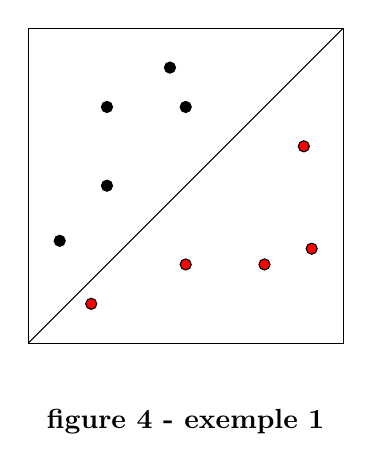
\begin{tikzpicture}[]
	%\draw[help lines, thick] (0,0) grid (4,4);
	\draw (0,0) rectangle (4,4);
	\filldraw (1,3) circle (2pt);
	\filldraw (2,3) circle (2pt);
	\filldraw (1,2) circle (2pt);
	\filldraw (0.4,1.3) circle (2pt);
	\filldraw (1.8,3.5) circle (2pt);
	\draw (0,0) -- (4,4);
	\filldraw (2,1) [fill=red] circle (2pt);
	\filldraw (3,1) [fill=red] circle (2pt);
	\filldraw (3.5,2.5) [fill=red] circle (2pt);
	\filldraw (3.6,1.2) [fill=red] circle (2pt);
	\filldraw (0.8,0.5) [fill=red] circle (2pt);
	\draw (2,-1) node { \textbf{figure 4 - exemple 1} };
\end{tikzpicture}
\end{center}
\vfill


Pour cela nous allons introduire un réseau de neurone composé d'une unité de type Sigmoid.
Ce neurone aura pour entrées les coordonnées du point choisit et pour sortie la valeur de la fonction d'activation qui est définit comme suit: 
\[ \frac{1}{1+e^{-w_{1}u-w_{2}v+\theta}}. \]

\vfill
\begin{center}
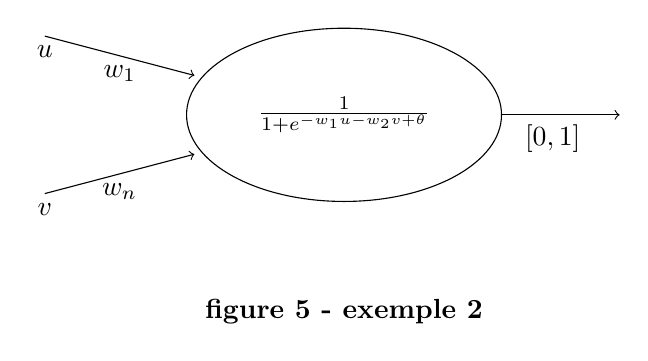
\begin{tikzpicture}[]
	%\draw[help lines, thick] (0,0) grid (9,5);
	\draw[->] (6.5,2.5)-- node[below, align=center] {$\left[0,1\right]$} (7.8,2.5)-- (8,2.5);
	\draw[->] (0.7,3.5) node [below] {$u$} -- node [below] {$w_{1}$} (2.6,3);
	\draw[->] (0.7,1.5) node [below] {$v$}-- node [below] {$w_{n}$} (2.6,2);
	\draw (4.5,2.5) node {$ \frac{1}{1+e^{-w_{1}u-w_{2}v+\theta}}  $} circle [x radius= 2, y radius=1.1];
	\draw (4.5,0) node { \textbf{figure 5 - exemple 2} };
\end{tikzpicture}
\end{center}
\vfill

Nous définissons la fonction $\Phi_{x}(w_{1},w_{2},\theta)= \frac{1}{1+e^{-w_{1}u-w_{2}v+\theta}}$ avec $x=(u,v)$.
Soit $E$ un ensemble de triplet dont chaque triplet est définit de la manière suivante : 
$x = (u,v,p)$ 	avec $u$ et $v$ l'abscisse et l'ordonnée du point $x$ et $p$ sa position par rapport à la droite $d$.

	\[ \begin{cases} 0 &\mbox{Si  p est en dessous de d } \\
				 0.5 & \mbox{Si p est sur d } \\
				 1 & \mbox{Si p est au dessus de d }
	 		 \end{cases} \] \\
Soit $ C_x(w_{1},w_{2},\theta) = \frac{1}{2}(y(x)-\Phi_x(w_{1},w_{2},\theta))^{2} $ la fonction de coût de $N$ avec $y(x)=p$.
Il suffit maintenant de calculer le gradient de la fonction $\gamma$ afin d'appliquer l'algorithme du Gradient pour que le réseau $N$ nous donne des valeurs proches de la réalité.\\
%************************************************** fin de l'exemple *****************************************************************
\newline

%faire l'exemple avec le neuronne et la droite de point, et faire une transition avec la retropropagation
\subsection{Rétropropagation}
Nous avons vu dans la partie précédente, comment nous pouvons minimiser la fonction $\gamma$ à condition d'avoir son gradient. Cette étape
devient très vite fastidieuse lorsque le réseau de neurone est formé de plusieurs couches de plusieurs neurones, car la fonction qui
définira ce réseau sera la composée de toutes les fonctions définissant les neurones contenu dans celui-ci. Ce problème va être résolue 
grâce à la rétropropagation qui est une méthode qui va nous permettre de calculer le gradient de n'importe quelle réseau.

\subsection {B-Diagramme}
Pour parler de la rétropropagation  nous nous devons d'introduire une nouvelle structure qui est le B-Diagramme (Backpropagation diagramme).
Ce diagramme représente les neurones utilisés dans notre réseau mais dans lesquelles nous stockons dans leurs partie gauche la valeur de la dérivée de leurs fonction et dans leurs partie droite la valeur de leurs fonction pour une entrée donnée.\\
\newline
% préciser les dérivéees partielle dans le diagramme
%************************************************** début de la figure *****************************************************************
\vfill
\begin{center}
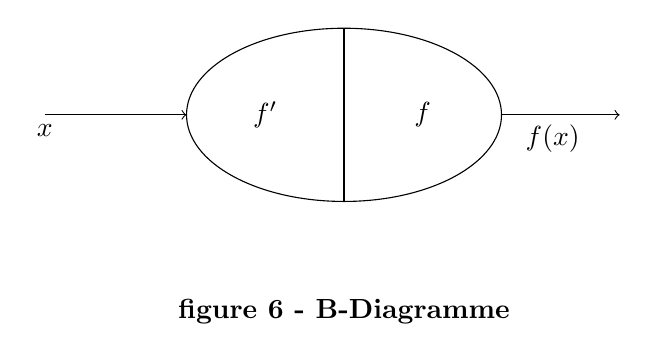
\begin{tikzpicture}[]
	%\draw[help lines, thick] (0,0) grid (9,5);
	\draw[->] (0.7,2.5) node [below] {$x$}-- (2.5,2.5);
	\draw[->] (6.5,2.5)-- node[below, align=center] {$f(x)$} (7.8,2.5)--(8,2.5);
	\draw (4.5,1.4)--(4.5,3.6);	
	\draw (4.5,2.5) circle [x radius= 2, y radius=1.1];
	\draw (3.5,2.5) node { $f'$ };
	\draw (5.5,2.5) node { $f$ };
	\draw (4.5,0) node { \textbf{figure 6 - B-Diagramme} };
\end{tikzpicture}
\end{center}
\vfill
%************************************************** fin de la figure *****************************************************************
 
La rétropropagation ce divise en deux étapes :
\begin{enumerate}
\item L'étape de feed-forward : Cette étape consiste à parcourir notre réseau de gauche à droite afin de calculer pour chaque neurone, la valeur de sa fonction et de sa dérivée pour une valeur donnée. Une fois calculé et comme dit précédemment chaque valeurs seront stockées dans leurs côté respective. Le résultat stocké à droite sera ensuite transmit au nœud suivant et le processus sera réitéré. % la régle avec leur et leurs
\item L'étape de rétropropagation : Dans cette étape le réseau sera parcouru de droite à gauche et la valeur stockée à gauche sera 
utilisée. Cette étape est divisée en plusieurs cas :
\begin{enumerate}
\item La composition  : Le réseau prend en entrée la constante 1. Celle-ci est multipliée par la valeur stockée dans la partie gauche du neurone. Le résultat sera ensuite transmis à l'unité suivante dans laquelle la constante sera multipliée par sa valeur de gauche. Le résultat final sera alors égale à $f'(g(x)).g'(x)$.
%************************************************** début de la figure *****************************************************************
\vfill
\begin{center}
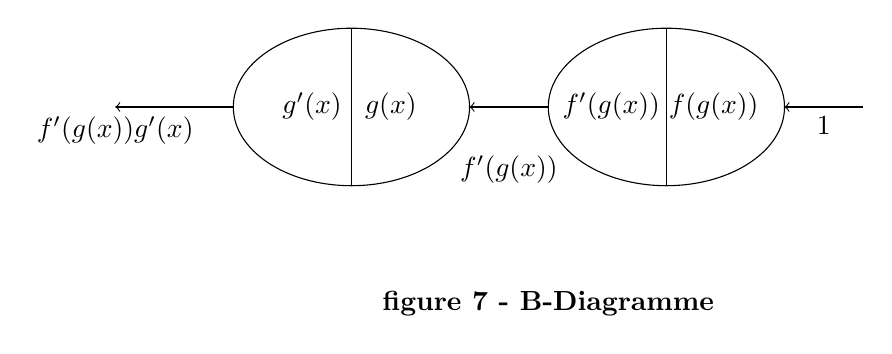
\begin{tikzpicture}[]
	%\draw[help lines, thick] (-1,0) grid (9,5);
	\draw[<-] (-1,2.5) node [below] {$f'(g(x))g'(x)$} -- (0.5,2.5);
	\draw[<-] (7.5,2.5)-- node [below] {$1$}(8.5,2.5);
	\draw[<-] (3.5,2.5) --(4.5,2.5);
	\draw (4,2) node [below] {$f'(g(x))$};
	\draw (2,3.5)--(2,1.5);
	\draw (6,3.5)--(6,1.5);
	\draw (2,2.5) circle [x radius= 1.5, y radius=1];
	\draw (6,2.5) circle [x radius= 1.5, y radius=1];
	\draw (1.5,2.5) node {$g'(x)$};
	\draw (2.5,2.5) node {$g(x)$};
	\draw (5.3,2.5) node {$f'(g(x))$};
	\draw (6.6,2.5) node {$f(g(x))$};
	\draw (4.5,0) node { \textbf{figure 7 - B-Diagramme} };
\end{tikzpicture}
\end{center}
\vfill
%************************************************** fin de la figure *****************************************************************
\item L'addition : Le réseau prend en entrée la constante 1, qui sera ensuite distribuée dans chaque unité. Lorsque deux unités se rencontre on additionne le résultat 
%************************************************** début de la figure *****************************************************************
\vfill
\begin{center}
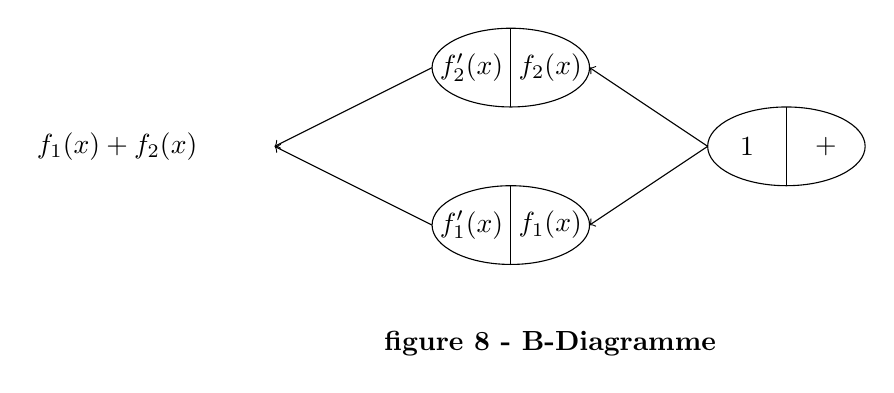
\begin{tikzpicture}[]
	%\draw[help lines, thick] (0,0) grid (9,5);
	\draw [<-] (5,1.5)--(6.5,2.5);
	\draw [<-] (5,3.5)--(6.5,2.5);
	\draw [->] (3,1.5)--(1,2.5);
	\draw [->] (3,3.5)--(1,2.5);
	\draw  (4,1)--(4,2);
	\draw  (4,3)--(4,4);
	\draw  (7.5,3)--(7.5,2);
	\draw (-1,2.5) node {$f_{1}(x)+f_2(x)$};
	\draw (3.5,1.5) node {$f'_{1}(x)$};
	\draw (3.5,3.5) node {$f'_2(x)$};
	\draw (4.5,1.5) node {$f_{1}(x)$};
	\draw (4.5,3.5) node {$f_2(x)$};
	\draw (8,2.5) node {$+$};
	\draw (7,2.5) node {$1$};
	\draw (4,1.5) circle [x radius= 1, y radius=0.5];
	\draw (4,3.5) circle [x radius= 1, y radius=0.5];
	\draw (7.5,2.5) circle [x radius= 1, y radius=0.5];
	\draw (4.5,0) node { \textbf{figure 8 - B-Diagramme} };
\end{tikzpicture}
\end{center}
\vfill
%************************************************** fin de la figure *****************************************************************
\item Les entrées avec poids :
\vfill
\begin{center}
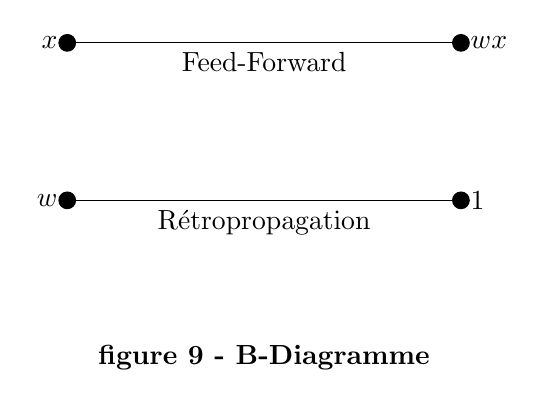
\begin{tikzpicture}[]
	%\draw[help lines, thick] (0,0) grid (9,5);
	\filldraw (2,2)[fill=black] circle (3pt);
	\draw (2,2)[left] node {$w$};
	\filldraw (7,2) [fill=black] circle (3pt);
	\draw (7,2)[right] node {$1$};
	\draw (2,2)--(7,2);
	\filldraw (2,4) [fill=black] circle (3pt);
	\draw (2,4)[left] node {$x$};
	\filldraw (7,4) [fill=black] circle (3pt);
	\draw (7,4)[right] node {$wx$};
	\draw (4.5,2) node [below] {Rétropropagation};
	\draw (4.5,4) node [below] {Feed-Forward};
	\draw (2,4)--(7,4);
	\draw (4.5,0) node { \textbf{figure 9 - B-Diagramme} };
\end{tikzpicture}
\end{center}
\vfill
\end{enumerate}
\end{enumerate}
\newpage
\section{Réseau de neurone et résolution de formule booléenne quantifiée}
Dans la partie précédente nous avons vu comment un réseau de neurone pouvait être entrainé et ainsi devenir plus performant. Dans cette partie, nous allons voir comment nous pouvons entrainer un réseau de neurone afin que celui-ci puisse résoudre des formules booléennes quantifiées.
Afin qu'un réseau de neurone puisse résoudre une formule booléenne quantifiée, il faut que celle-ci soit mise sous forme prénexe.
\subsection{Définition : Forme prénexe}
	On dit que une formule et sous forme prénexe si tout ses quantificateurs existentiels et universels sont placés au début de la formule. 
	\[ G= Q_{1}x_{1}Q_{2}x_{2}....Q_{n}x_{2}G' \] avec $G'$ une formule booléenne sans quantificateur.
\newline \\
Afin de résoudre une formule quantifiée, on utilisera deux réseaux de neurone qui s'affronteront dans un jeu dont les règles sont les suivante : 
	%% à compléter
	%% Développer le jeu 

Les deux réseaux de neurone que nous utilisons sont constitués de la même façon. Leur constitution est donnée par le schéma suivant.

%% Exprime le réseau de neurone qu'on a 
\begin{center}
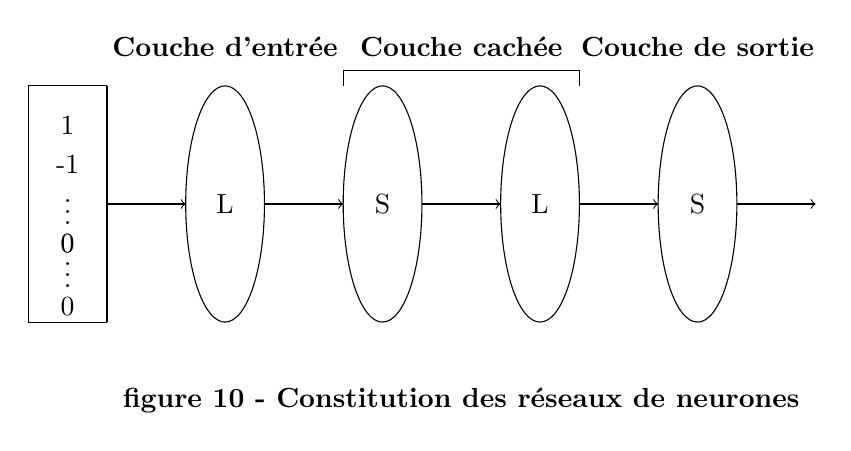
\begin{tikzpicture}[]
	%\draw[help lines, thick] (0,0) grid (11,5);
	\draw (2.5,2.5) node {L} circle [x radius=0.5, y radius=1.5];
	\draw (4.5,2.5) node {S} circle [x radius=0.5, y radius=1.5];
	\draw (6.5,2.5)node{L}circle[x radius=0.5, y radius=1.5];
	\draw (8.5,2.5) node {S} circle [x radius=0.5, y radius=1.5];
	\draw [->] (3,2.5)--(4,2.5);
	\draw [->] (1,2.5)--(2,2.5);
	\draw [->] (5,2.5)--(6,2.5);
	\draw [->] (7,2.5)--(8,2.5);
	\draw (0,4)--(1,4);
	\draw (0,4)--(0,1); 
	\draw (1,4)--(1,1); 
	\draw (0,1)--(1,1);
	\draw (4,4)--(4,4.2);
	\draw (7,4)--(7,4.2);
	\draw (4,4.2)--(7,4.2);
	\draw (0.5,3.5) node{1};
	\draw (0.5,3) node{-1};
	\draw (0.5,2.5) node{\vdots};
	\draw (0.5,2) node{0};
	\draw (0.5,1.7) node{\vdots};
	\draw (0.5,2) node{0};
	\draw (0.5,1.2) node{0};
	\draw [->] (9,2.5)--(10,2.5);
	\draw (2.5,4.5) node {\textbf{Couche d'entrée}}; 
	\draw (5.5,4.5) node {\textbf{Couche cachée}}; 
	\draw (8.5,4.5) node {\textbf{Couche de sortie}}; 
	\draw (5.5,0) node { \textbf{figure 10 - Constitution des réseaux de neurones }};
\end{tikzpicture}
\end{center}
\end{document} 
